\documentclass[apj]{emulateapj}
\usepackage{amsmath}
\shorttitle{Unstable $\MakeLowercase{m} = 1$ Eccentric Modes }
\shortauthors{Dempsey \& Lithwick}
\begin{document}
\title{Unstable $\MakeLowercase{m} = 1$ Eccentric Modes in Thermally Cooling, Self Gravitating Disks}
\author{Adam M. Dempsey \& Yoram Lithwick}
\affil{Center for Interdisciplinary Exploration and Research in Astrophysics (CIERA)
and
Department of Physics and Astronomy
Northwestern University
2145 Sheridan Road
Evanston, IL 60208
USA}
\email{adamdempsey2012@northwestern.edu}


\begin{abstract}


\end{abstract}


\section{Introduction}

\section{Equations of Motion}
The equations of motion for a two dimensional, viscous disk are
\begin{equation}
(\partial_t + \mathbf{v} \cdot \mathbf{\nabla}) \mathbf{v} = - \frac{ \mathbf{\nabla} P}{\Sigma} - \mathbf{\nabla}\Phi + \frac{1}{\Sigma} \mathbf{\nabla} \cdot ( \nu \Sigma \mathbf{D} )
\end{equation}
\begin{equation}
(\partial_t + \mathbf{v} \cdot \mathbf{\nabla}) \Sigma = - \Sigma \mathbf{\nabla} \cdot \mathbf{v}
\end{equation}
\begin{equation}
T (\partial_t + \mathbf{v} \cdot \mathbf{\nabla} ) s = - \frac{ T - \bar{T}}{t_\text{cool}}
\end{equation}
Where all quantities are assumed to be a vertical average of their three dimensional counterparts. Here, $\Sigma$ is the surface density, $s$ is the entropy of the fluid, $T$ is the disk temperature, and $\mathbf{D}$ is the viscous stress tensor. These equations describe a viscous fluid that is thermally heated and or cooled to some "background" temperature profile $\bar{T}$ over a timescale $t_\text{cool}$. To close the system of equations we assume the fluid is ideal and perfect, so that $P =  \mathcal{R} \Sigma T $ and $s \equiv \frac{\mathcal{R}}{\gamma -1} \ln \left( P \Sigma^{-\gamma} \right)$; hereafter we set $\mathcal{R} =1$ without loss of generality. Following \citet{osa92}, we can connect the two dimension adiabatic index $\gamma$ to the true three dimensional adiabatic index $\Gamma$ by assuming that the gas is vertically isothermal and gaussian distributed. 

We consider a disk with a prescribed azimuthally averaged background profile given by $(\bar{v}_r, \bar{v}_\phi, \bar{\Sigma}, \bar{T}) = ( 0, r \Omega(r), \bar{\Sigma} \propto r^\mu, \bar{T} \propto r^\delta) $. We look at linear perturbations to this background state. Denoted linear quantities with a prime and background quantities with a bar, the linearized equations of motion become
\begin{equation}
(\partial_t + \Omega \partial_\phi) v_r' - 2\Omega v_\phi' = - \frac{1}{\bar{\Sigma}} \partial_r P' + \frac{\Sigma'}{\bar{\Sigma}^2} \frac{d \bar{P}}{d r} - \partial_r \Phi' + \text{visc.}
\end{equation}
\begin{equation}
(\partial_t + \Omega \partial_\phi) v_\phi' + \frac{\kappa^2}{2\Omega} v_r' = - \frac{1}{r \bar{\Sigma}} \partial_\phi P'  -\frac{1}{r} \partial_\phi \Phi' + \text{visc.}
\end{equation}
\begin{equation}
(\partial_t + \Omega \partial_\phi)  \Sigma'  + v_r' \frac{ d \bar{\Sigma}}{d r }= - \bar{\Sigma} \left( \frac{1}{r} \partial_r ( r v_r') + \frac{1}{r} \partial_\phi(v_\phi' ) \right)
\end{equation}
\begin{equation}
(\partial_t + \Omega \partial_\phi)  s' +  v_r' \frac{d \bar{s}}{d r}  = - \beta \Omega \frac{T'}{\bar{T}}
\end{equation}
Where we've parametrized the cooling time as $t_\text{cool}^{-1} = \beta \Omega $ \citep{gam01}. We now Fourier Transform the linear variables in the azimuthal direction as well as in time and write $(v_r',v_\phi',\Sigma', P', s', T' , \Phi') = \sum_m  (u,v,\sigma,p,s,T,\phi) e^{ i  m(\phi -  \Omega_p t) } $. We further work under the assumption that the different $m$ modes only couple to the $m=0$ mode (i.e the background) and not to other $m \neq 0$ modes. The linearized equations of motion are now
\begin{equation}
i m (\Omega - \Omega_p) u - 2 \Omega v  = - \frac{1}{\bar{\Sigma}} \frac{d p}{d r} + \frac{\sigma}{\bar{\Sigma}^2} \frac{d \bar{P}}{d r} - \frac{ d \phi}{d r} + \text{visc.}
\end{equation}
 \begin{equation}
i m (\Omega - \Omega_p) v + \frac{\kappa^2}{2 \Omega} u  = - \frac{i m p}{r \bar{\Sigma}}  - \frac{ i m \phi}{ r} + \text{visc.}
\end{equation}
\begin{equation}  \label{eq:dtsigma}
i m (\Omega - \Omega_p) \frac{ \sigma }{ \bar{\Sigma}}+ u \frac{d \ln \bar{\Sigma}}{d r} = - \left( \frac{1}{r} \frac{d }{d r} ( r u) + \frac{ i m v}{r } \right)
\end{equation}
\begin{eqnarray}  \label{eq:dtT}
i m \left[ \left( 1 - i \frac{\beta(\gamma -1)}{m} \right) \Omega - \Omega_p \right] \frac{T'}{\bar{T} } &+& u \frac{d  \ln \bar{T}}{d r}   \\ 
&=& -(\gamma -1)  \left( \frac{1}{r} \frac{d }{d r} ( r u) + \frac{ i m v}{r } \right) \nonumber
\end{eqnarray}
Where we've replaced the entropy in favor of the temperature through the relations
\begin{equation}
(\gamma -1)s' = \frac{ T'}{ \bar{T}} - (\gamma -1 ) \frac{ \sigma}{ \bar{\Sigma}} 
\end{equation}
\begin{equation}
(\gamma -1)\frac{d \bar{s}}{d r} = \frac{d \ln \bar{T}}{d r} - (\gamma -1) \frac{ d \ln \bar{\Sigma}}{d r} 
\end{equation}


\section{ $\MakeLowercase{m}=1$ Slow Modes }
We specialize to $m=1$ modes and to the low pattern speed limit $\Omega_p \ll \Omega$. We can simplify the 4 dimensional set of equations to just one equation describing the global structure and evolution of an eccentricity vector, $e(r)$ \citep{og01,go06,papa02}. The eccentricity is defined through the Lagrangian displacement $\xi_r$ as 
\begin{equation}
e \equiv \frac{ \xi_r} {r} 
\end{equation}
 Following \cite{papa02} we can write an evolution equation for the disk eccentricity by an appropriate linear combination of the two momenta equations and using 
 \begin{equation}
2 \Omega r^3 ( \Omega_p - \omega_p) e = - \frac{d }{dr} \left( r^2 \frac{p}{\bar{\Sigma}} \ + r^2 \phi \right) + \frac{r^2}{\bar{\Sigma}^2} \left[  \sigma \frac{ d \bar{P}}{d r}-p \frac{d \bar{\Sigma}}{d r} \right]
\end{equation}
\begin{equation} \label{eq:wp_def}
2 \Omega r^3 \omega_p = - r \frac{d}{dr} \left( \frac{r^2}{\bar{\Sigma}} \frac{d \bar{P}}{d r} \right) - r \frac{ d}{dr} \left( r^2 \frac{d \bar{\Phi}}{dr} \right)
\end{equation}

 \begin{equation}
p = \sigma \bar{T} + \bar{\Sigma} T'
\end{equation}
 \begin{equation}
\frac{\sigma}{\bar{\Sigma}} = - \frac{d \ln \bar{\Sigma}}{ d \ln r} e - r \frac{d e}{d r} 
\end{equation}
\begin{equation}
(1- i\tilde{\beta}) \frac{T'}{\bar{T}} = -\frac{d \ln \bar{T}}{d \ln r} e - (\gamma -1) r \frac{d e}{d r}
\end{equation}

\subsection{No Cooling} 

We define the  adiabatic limit as when $\beta=0$, the eccentricity equation in this limit reduces to,
\begin{equation}
2 \Omega r^3 ( \Omega_p - \omega_p) e = - \frac{d}{dr} \left( \frac{r^2 p}{\bar{\Sigma}} + r^2 \phi \right) + \frac{r^2}{\bar{\Sigma}} \left( \sigma \frac{d \bar{P}}{dr} - p \frac{d \bar{\Sigma}}{d r} \right) 
\end{equation}
\begin{equation}
\frac{p}{\bar{P}} = - \frac{ d\ln \bar{P}}{d \ln r } e - \gamma r \frac{ d e}{d r}
\end{equation}
This is equivalent to the eccentricity equation of e.g \citet{go06} (their Eq. 21), when we use \eqref{eq:wp_def} to replace $\omega_p$. 

We define the barotropic limit as when $\gamma \rightarrow 1$ and we can write the total pressure as $P = P(\Sigma)$. We then define the sound speed $c^2$, such that, $p = c^2 \sigma$ and $\frac{d \bar{P}}{d \bar{\Sigma}} = c^2 $. The eccentricity equation simplifies in this case to,
\begin{equation}
2 \Omega r^3 ( \Omega_p - \omega_p) e = - \frac{d}{dr} \left( r^2 \frac{c^2 \sigma}{\bar{\Sigma}} + r^2 \phi \right) 
\end{equation}
This is equivalent to the eccentricity equation of e.g \citet{papa02} (his Eq. 18).

The locally isothermal limit is defined as $\gamma \rightarrow 1$ and $P = \bar{T}(r) \Sigma$. The eccentricty equation in the locally isothermal limit is then,
\begin{equation}
2 \Omega r^3 ( \Omega_p - \omega_p) e = - \bar{T} \frac{d}{dr} \left( r^2 \frac{\sigma}{\bar{\Sigma}} \right) - \frac{d}{dr} \left( r^2 \phi \right) 
\end{equation}
This is equivalent to the linear system that e.g, \citet{lin15} studied. 
 
\subsection{With Cooling}



Which follow from \eqref{eq:dtsigma} \& \eqref{eq:dtT} to zeroth order in $\Omega_p$ and with $\Omega \approx \Omega_K$. We obtain the evolution equation 
\begin{equation} \label{eq:coeff_eqn}
\Omega_p e  = A e + B \frac{d e}{d \ln r} + C  \frac{d^2 e}{ d \ln r^2}
\end{equation}
Where the coefficients are,
\begin{equation}
A = \omega_p  + \mathcal{H} \left[ 2 \mu + \mu'  + \frac{1}{1 - i  \tilde{\beta}} ( \delta' + \delta (2 + \mu + \delta) \right]
\end{equation}
\begin{equation}
B = \mathcal{H} \left[ 2 + \mu + \frac{1}{1 - i \tilde{\beta}} ( \left( \gamma \delta + (\gamma -1 ) (2 + \mu) \right) \right]
\end{equation}
\begin{equation}
C = \mathcal{H} \left[ 1 +  \frac{(\gamma - 1)}{1 - i  \tilde{\beta}} \right]
\end{equation}
Where,
\begin{equation}
\tilde{ \beta} \equiv \beta ( \gamma - 1)
\end{equation}
\begin{equation}
\mathcal{H} \equiv \frac{  \bar{T}}{ 2 \Omega r^2}
\end{equation}
\begin{equation}
\mu ' = \frac{d ^2 \bar{\Sigma}}{d \ln r^2} 
\qquad \qquad
\delta' = \frac{d ^2 \bar{T}}{d \ln r^2}
\end{equation}
To add in the effects of viscosity we first use the alpha parametrization of viscosity and take $\nu = \alpha \frac{T}{\Omega}$ \citep{ss73}. The corrections due to shear ($\alpha_s$) and bulk ($\alpha_b$) viscosities are, 
\begin{equation}
A_\nu = -\frac{i \alpha_s}{6} \mathcal{H} \left( \frac{65}{2} + \delta - 2 \mu + 18 \mu' \right)
\end{equation}
\begin{equation}
B_\nu = -\frac{ i \alpha_s}{3} \mathcal{H} \left( -\frac{19}{2} - 7 \delta + 2 \mu \right) +  i \alpha_b \mathcal{H} \left( \frac{5}{2} + \delta + \mu \right)
\end{equation}
\begin{equation}
C_\nu = - \frac{ i 2\alpha_s}{3} \mathcal{H}  - i \alpha_b \mathcal{H}
\end{equation}



We solve \eqref{eq:coeff_eqn} as a generalized eigenvalue problem by discretizing the eccentricity on a logarithmic grid in radius. 
\begin{equation}
\Omega_p \mathbf{Q} \mathbf{e} = \mathbf{M} \mathbf{e}
\end{equation}
The matrices $\mathbf{Q}$, and $\mathbf{M}$ are the boundary condition matrix and the coefficient matrix, respectively. We solve for the spectrum of normal eigenmodes, $\mathbf{e}_n$ and their associated (possibly complex) eigenvalues $\Omega_{p,n}$. 








\subsection{Boundary Condition} 
We adopt a zero Lagrangian pressure boundary condition at both the inner and outer boundaries. Using the equations of motion it can be shown that this is equivalent to satisfying 
\begin{equation}
%\left. r \frac{d e(r) }{d r}\right|_{r_i, r_o} = \left. \left[ \frac{ \beta^2}{\gamma^2 + \beta^2} - i \frac{ \gamma \beta}{\gamma^2 + \beta^2} \right] \frac{d \ln \bar{T}}{d \ln r } e(r) \right|_{r_i, r_o}
\left. r \frac{d e(r) }{d r}\right|_{r_i, r_o} = \left. \tilde{\beta} \left[ \frac{ \tilde{\beta} - i \gamma }{ \tilde{\beta}^2 + \gamma^2 } \right] \frac{d \ln \bar{T}}{d \ln r } e(r) \right|_{r_i, r_o}
\end{equation}
at each boundary in the slow mode approximation. In the isothermal ($\beta \rightarrow \infty$) and adiabatic ($\beta \rightarrow 0$) limits the boundary condition reduces to,
\begin{equation}
\left. r \frac{d e(r)}{d r} \right|_{r_i, r_o} = 
\begin{cases}
\left. \frac{d \ln \bar{T}}{d \ln r} e(r) \right|_{r_i,r_o}  & \text{Isothermal} \\ \\ 
0 & \text{Adiabatic}
\end{cases}
\end{equation}


\section{Methods}


\section{Results}
We studied the growth rates of unstable modes in the slow mode ($\Omega_p \ll \Omega_k$) approximation. The classical WKB dispersion relation for a self gravitating and isothermal disk (see e.g \citet{bt2}) is
\begin{equation}
 \kappa^2  - m^2 \varpi^2 - 2 \pi G \Sigma |k_r| + c^2 k_r^2  = 0
\end{equation}
Where $\varpi \equiv \Omega - \Omega_p$. In the $m=1$ slow mode limit this simplifies to \citep{papa02}
\begin{equation}
2 \Omega ( \Omega_p - \omega_p) =  2 \pi G \Sigma |k_r| - c^2 k_r^2 
\end{equation}
Where $\omega_p = \Omega - \kappa$ is the orbital precession frequency of a fluid element. From the dispersion relation it is clear that pressure creates retrograde modes ($\Omega_p < 0$) and self gravity tends to create prograde modes ($\Omega_p > 0$). Additionally, global modes (i.e low $k_r$) also tend to create prograde modes \citep{papa02}. 

To understand the implications of cooling on the disk, we write the the WKB dispersion relation for a disk which has consonant cooling $\beta$ and constant background profiles. After some algebra, we obtain
\begin{equation}
 \kappa^2  - m^2 \varpi^2 - 2 \pi G \Sigma |k_r| + k_r^2 c_\text{cool}^2= 0
\end{equation}
\begin{equation}
c_\text{cool}^2 =  \frac{ m \varpi}{ m \varpi - i \tilde{\beta} \Omega} c_\text{adi}^2 - \frac{ i \tilde{\beta} \Omega }{ m \varpi - i \tilde{\beta} \Omega} c_\text{iso}^2
\end{equation}
In the $m=1$, slow mode limit we obtain
\begin{equation}
2 \Omega ( \Omega_p - \omega_p) = 2 \pi G \Sigma |k_r| - k_r^2 c_\text{cool}^2  
\end{equation}
\begin{equation}
c_\text{cool}^2 = \frac{1}{1 - i \tilde{\beta}} c_\text{adi}^2 + \frac{ i \tilde{\beta}}{i \tilde{\beta} -1 } c_\text{iso}^2
\end{equation}
Where $c_\text{adi}^2 = \gamma c_\text{iso}^2$ is the sound speed in the adiabatic ($\beta = 0$) limit. Figure  shows the dependence of the decay rate with $\beta$. 

\begin{figure}[h]
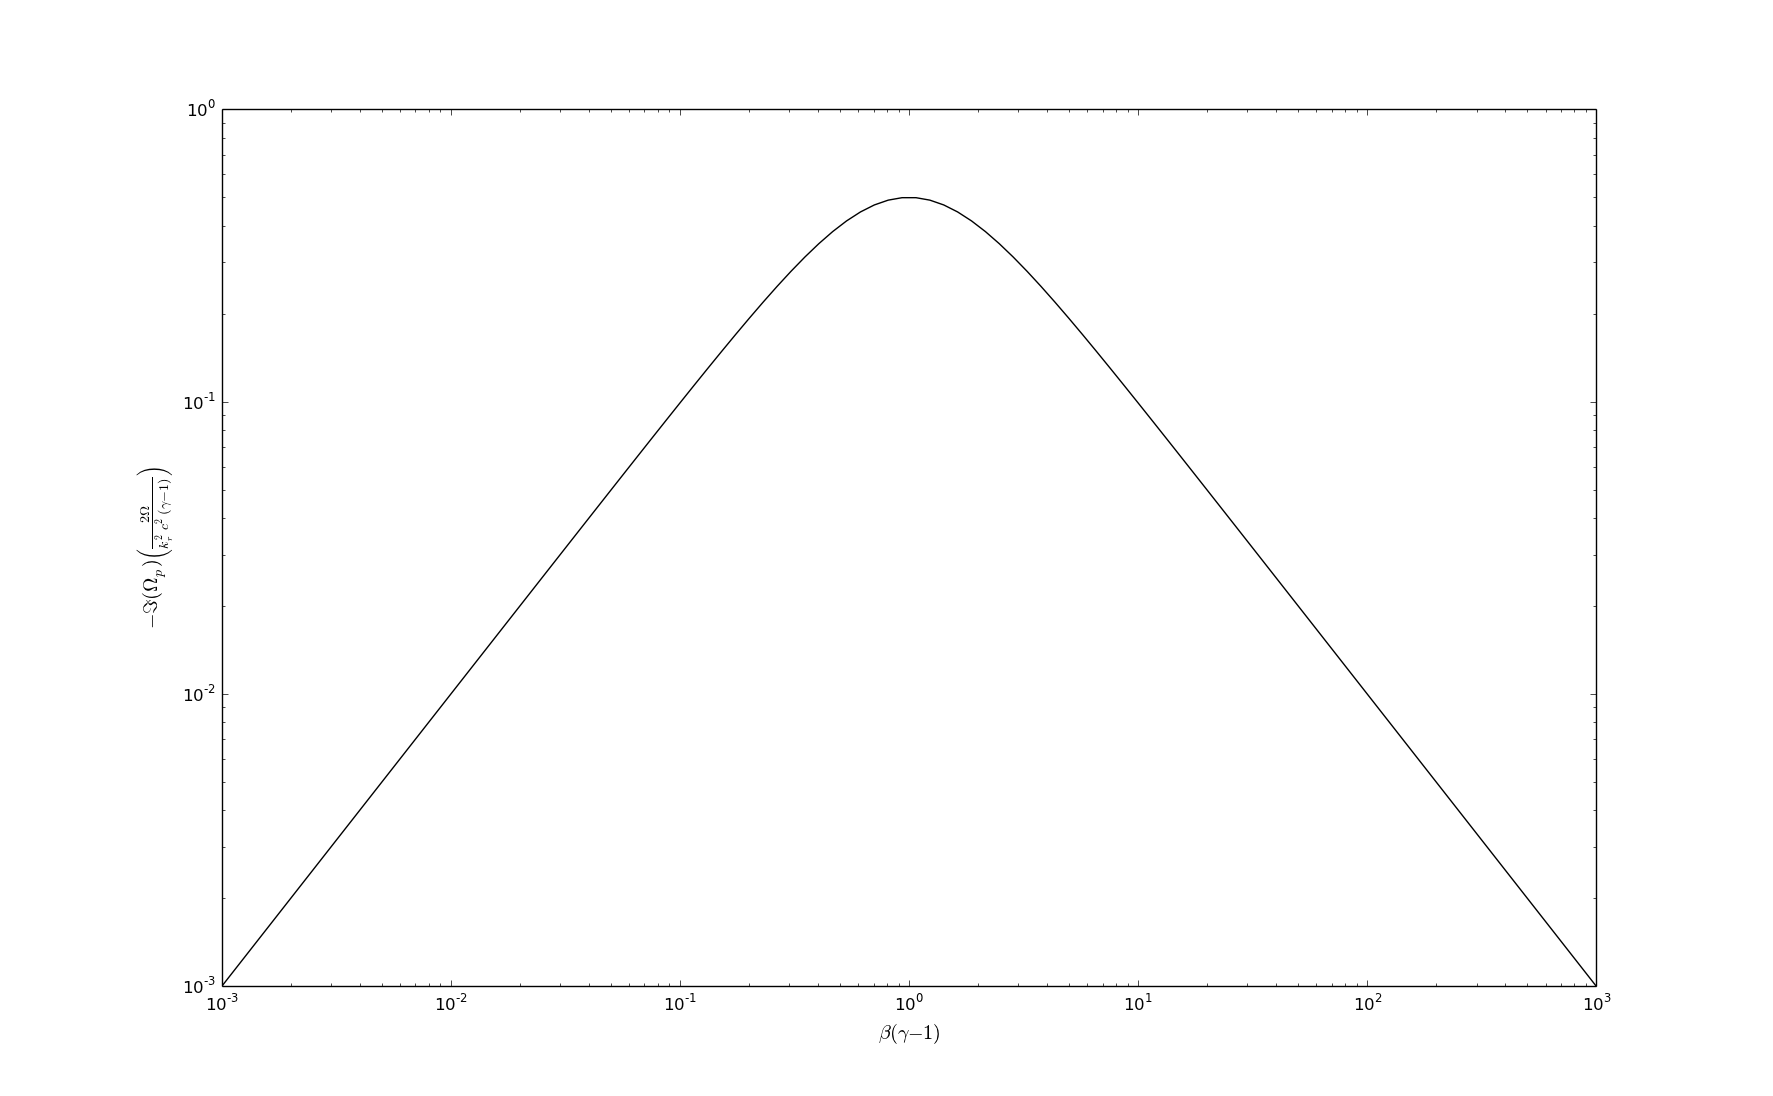
\includegraphics[width=.5\textwidth]{growth_wkb}
\caption{}
\end{figure}







\subsection{Lowest Order Mode with No Self Gravity}
The mode with zero nodes is perhaps the simplest to understand. 




\subsection{Self Gravity}

To include the effects of the disk's self gravity, we include the potential due to the perturbed surface density,

\begin{equation}
\phi' = - G \int dr' \, r' \Sigma'(r') \int d\phi \, \frac{\cos \phi}{\sqrt{ r^2 + r'^2 - 2 r r' \cos \phi}}
\end{equation}
The $\phi$ integral is simply the Laplace coefficient, $b_{1/2}^{(1)}$
\begin{equation}
b_{1/2}^{(1)} \left( \frac{ r'}{r} \right) = \frac{2}{\pi r} \int_0^\pi d\phi \,  \frac{\cos \phi}{\sqrt{1 + \left( \frac{r'}{r} \right)^2  - 2{\left( \frac{r'}{r} \right) \cos \phi}}}
\end{equation}
So that the potential is, 
\begin{equation} \label{eq:potential_integral_def}
\phi' = - \frac{ G \pi}{r} \int dr' \, r' \Sigma'(r') b_{1/2}^{(1)} \left( \frac{r'}{r} \right)
\end{equation}
There is also an "edge" contribution to the potential due to there being a non-negligable excess of material outside the outer boundary of the disk and a decificit of disk material inside the inner boundary of the disk. At the outer boundary of the disk we have, $\Sigma'(r) dr = \bar{\Sigma}(r_o) \xi_r(r_o) = \bar{\Sigma}(r_o) r_o e(r_o)$. Similarly at the inner boundary we have, $\Sigma'(r) dr' = - \bar{\Sigma}(r_i) \xi_r(r_i) = \bar{\Sigma}(r_i) r_i e(r_i)$. The "edge" potential is thus, 
\begin{equation}
\phi_\text{edge} = - \frac{G\pi \bar{\Sigma}(r_o) r_o^2 e(r_o)}{r}   b_{1/2}^{(1)} \left( \frac{r_o}{r} \right)  + \frac{G\pi \bar{\Sigma}(r_i) r_i^2 e(r_i)}{r}   b_{1/2}^{(1)} \left( \frac{r_i}{r} \right)
\end{equation}


The perturbed surface density is related to the eccentricity as $\phi' = - r \frac{d}{dr} \left( \bar{\Sigma} e \right)$. Plugging this in to \eqref{eq:potential_integral_def} and integrating by parts gives, 
\begin{equation}
\phi' = -\phi_\text{edge} - \frac{G \pi}{r} \int dr' \,  \bar{\Sigma}(r') e(r') \partial_{r'} \left( r'^2 b_{1/2}^{(1)} \left( \frac{r'}{r} \right) \right)
\end{equation}
The "edge" contribution to the potential thus cancels when we take $\phi' \rightarrow \phi' + \phi_\text{edge}$. The potential enters the eccentricity equation via the term,
\begin{equation}
- \frac{d}{dr} \left( r^2 \phi' \right)
\end{equation}


\section{Discussion}

\begin{equation}

\end{equation}





\section{Conclusions}

\begin{thebibliography}{}
\bibitem[Binney \& Tremaine(2002)]{bt2} Binney, J., Tremaine, S. \emph{Galactic Dynamics}. Princeton University Press, 2002.
\bibitem[Gammie 2001]{gam01} Gammie, C. F. (2001). \apj, 553(1), 174-183. 
\bibitem[Goodchild \& Ogilvie (2006)]{go06} Goodchild, S., \& Ogilvie, G. (2006). MNRAS, 368(3), 1123-1131. 
\bibitem[Lin(2015)]{lin15} Lin, M.-K.\ 2015, \mnras, 448, 3806 \bibitem[Ogilvie (2001)]{go01} Ogilvie, G. I. (2001). MNRAS, 325(1), 231-248. 
\bibitem[Ostriker, Shu, \& Adams (1992)]{osa92} Ostriker, E. C., Shu, F. H., \& Adams, F. C. (1992). \apj, 399, 192-212. 
\bibitem[Papaloizou(2002)]{papa02} Papaloizou, J. C. B. (2002). Astronomy and Astrophysics, 388(2), 615-631. 
\bibitem[Shakura \& Sunyaev(1973)]{ss73} Shakura, N. I., \& Sunyaev, R. A. (1973). Astronomy and Astrophysics, 24, 337?355.
\end{thebibliography}


\end{document}